\documentclass[a4paper, 12pt]{article}
\usepackage[a4paper,margin=2.5cm]{geometry}

%%%% Fontes e língua %%%%
\usepackage{fontspec}%for XeLaTeX, selecting multiple fonts
\usepackage{polyglossia}%for XeLaTeX, enables multiple languages.
\setmainlanguage{brazil}
\PolyglossiaSetup{brazil}{indentfirst=true}
\setotherlanguages{english}
\usepackage{csquotes}
\setmainfont[Ligatures=TeX]{Latin Modern Roman}
\setsansfont[Ligatures=TeX]{Latin Modern Sans}
\setmonofont{Latin Modern Mono}
\usepackage{amsmath, amsfonts, amssymb}
\renewcommand{\baselinestretch}{1.15}
%%%%%%%%%%%%%%%%%

\usepackage{xcolor}
\usepackage{enumerate}  % listas com numeração diferente

%%%% Gráficos, posicionamento de tabelas
\usepackage{graphicx}
\usepackage{float}
\floatstyle{plaintop} % tabelas com legenda na parte de cima
\restylefloat{table}  % tabelas com legenda na parte de cima

\usepackage{longtable}
\usepackage{booktabs}

\usepackage{caption} % figuras com subfiguras
\usepackage{subcaption}  % figuras com subfiguras
\graphicspath{{figuras/}}
%%%%%%%%

% style = <file>
% bibstyle = <file>
% citestyle = <file>

% original:
%\usepackage[style=numeric,backend=biber,sorting=none]{biblatex}

%\usepackage[style=chem-acs, backend=biber,sorting=none,hyperref=true]{biblatex}
%\addbibresource{library.bib}


%%%% Headers e footers %%%%
%\usepackage{fancyhdr}
%\pagestyle{fancy}
%\fancyhead{}
%\fancyfoot{}
%\fancyhead[L]{Relatório Anual 2017}
%\fancyhead[R]{Karl Jan Clinckspoor}
%\fancyfoot[C]{\thepage}
%\renewcommand{\footrulewidth}{0pt}
%\setlength{\headheight}{15pt} 
%%%%%

\usepackage{hyperref}

\title{Guia de instalação do Python e uso do script de tratamento de curvas de fluxo}
\author{Karl Jan Clinckspoor}
\date{\today}

\begin{document}

\maketitle

\tableofcontents

\section{Configuração do RheoWin}

O script necessita que os dados estejam em .txt. Isso pode ser feito de duas maneiras.

\begin{enumerate}
\item Exportando medidas já existentes pelo Data Manager
\item Configurando o Job Manager para automaticamente exportar os dados após a medida ter terminado
\end{enumerate}

\subsection{Exportar medidas existentes para ASCII}
Abra um arquivo no Data Manager. Configure as colunas para mostrarem $\dot{\gamma}$ (taxa de cisalhamento) e $\eta$ (viscosidade). Isso é feito clicando com o botão direito na coluna e depois escolhendo a medida relevante. Não importa a ordem ou se há medidas anteriores, desde que não haja mais de um local com valores de $\dot{\gamma}$ e $\eta$.

\begin{center}
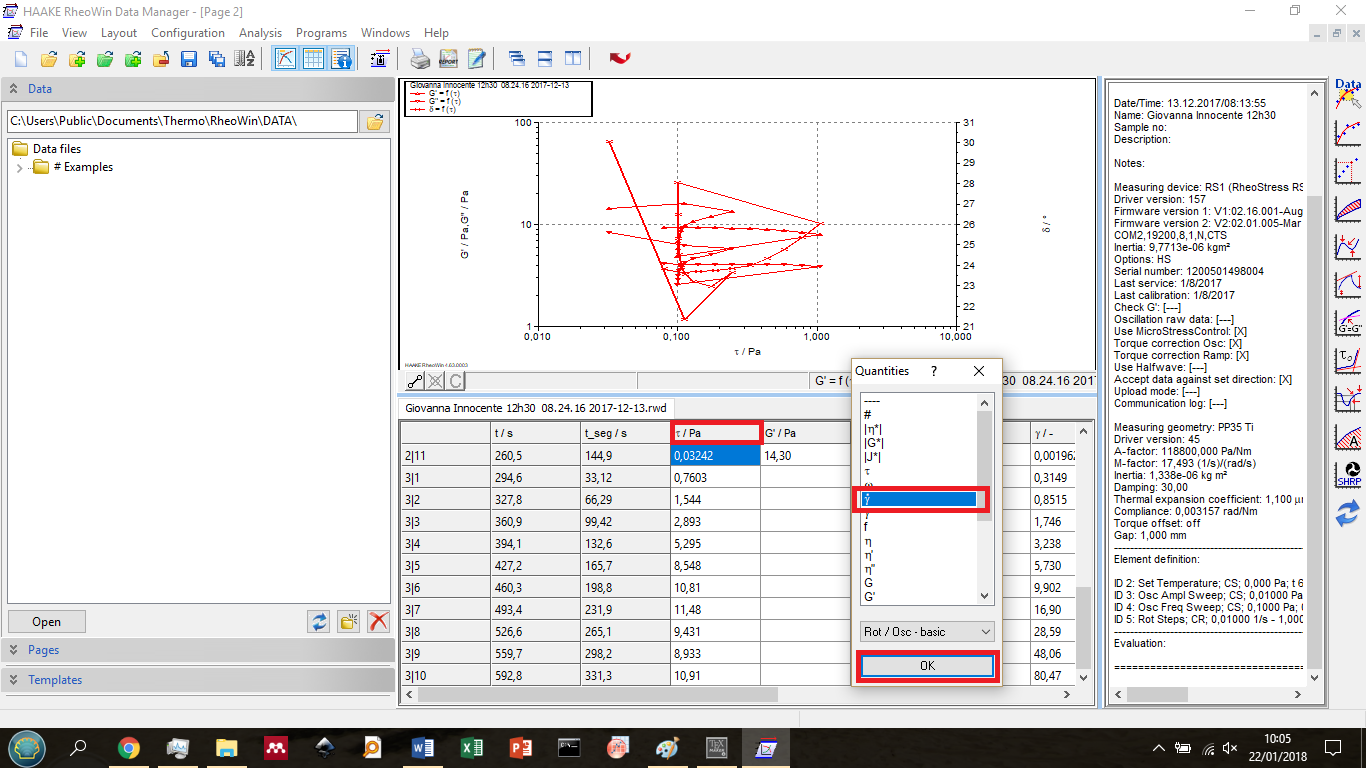
\includegraphics[width=0.80\textwidth]{DataMan1}
\end{center}

\begin{center}
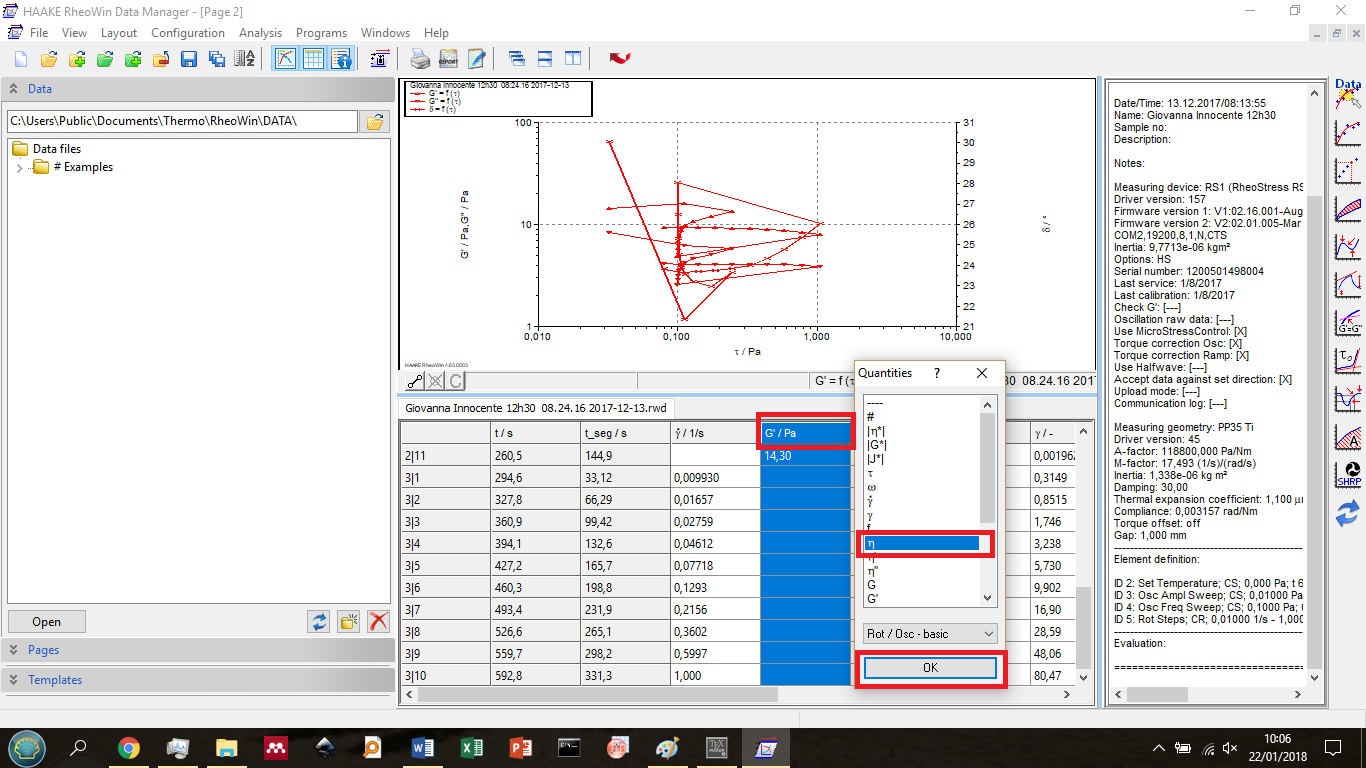
\includegraphics[width=0.8\textwidth]{DataMan2}
\end{center}

Após alterar as colunas, clique com o botão direito na aba com o nome da medida e clique em \texttt{Save to ASCII...}.

\begin{center}
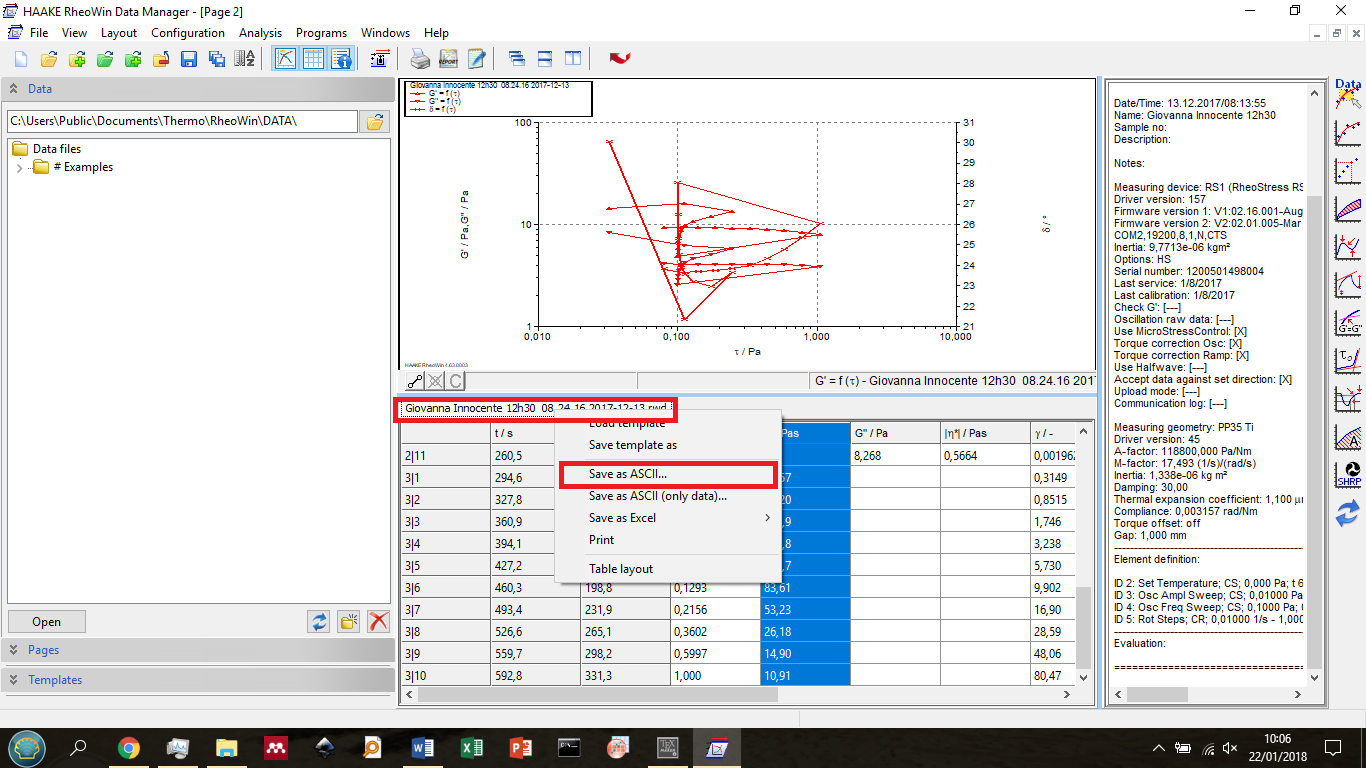
\includegraphics[width=0.8\textwidth]{DataMan3} 
\end{center}

Salve num local apropriado.

\subsection{Exportar para ASCII automaticamente}

Para novas medidas, é conveniente configurar o Job Manager para automaticamente converter as medidas em ASCII depois de terminada a análise. Isso é feito clicando-se, no Job, em \texttt{Filename}.

\begin{center}
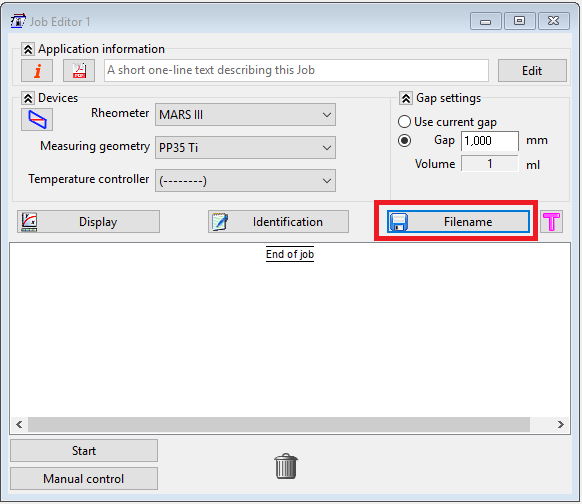
\includegraphics[width = 0.8\textwidth]{JobMan1}
\end{center}

Depois clique em \texttt{Save Table as ASCII file (*.txt)}.

\begin{center}
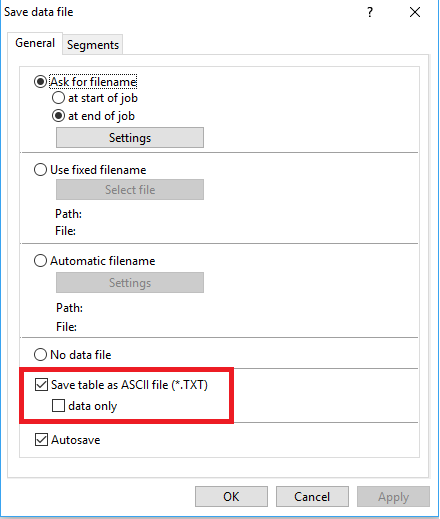
\includegraphics[width = 0.6\textwidth]{JobMan2}
\end{center}

Também é possível configurar o Job Manager para dar um nome automaticamente às amostras, com o horário e a data do dia, clicando em \texttt{Automatic Filename}, escolhendo o diretório base e configurando os parâmetros que irão no nome. É possível configurar para que o nome dado à amostra no início de cada medida se tornar o nome do arquivo no final, evitando de se escrever duas vezes o nome.

\begin{center}
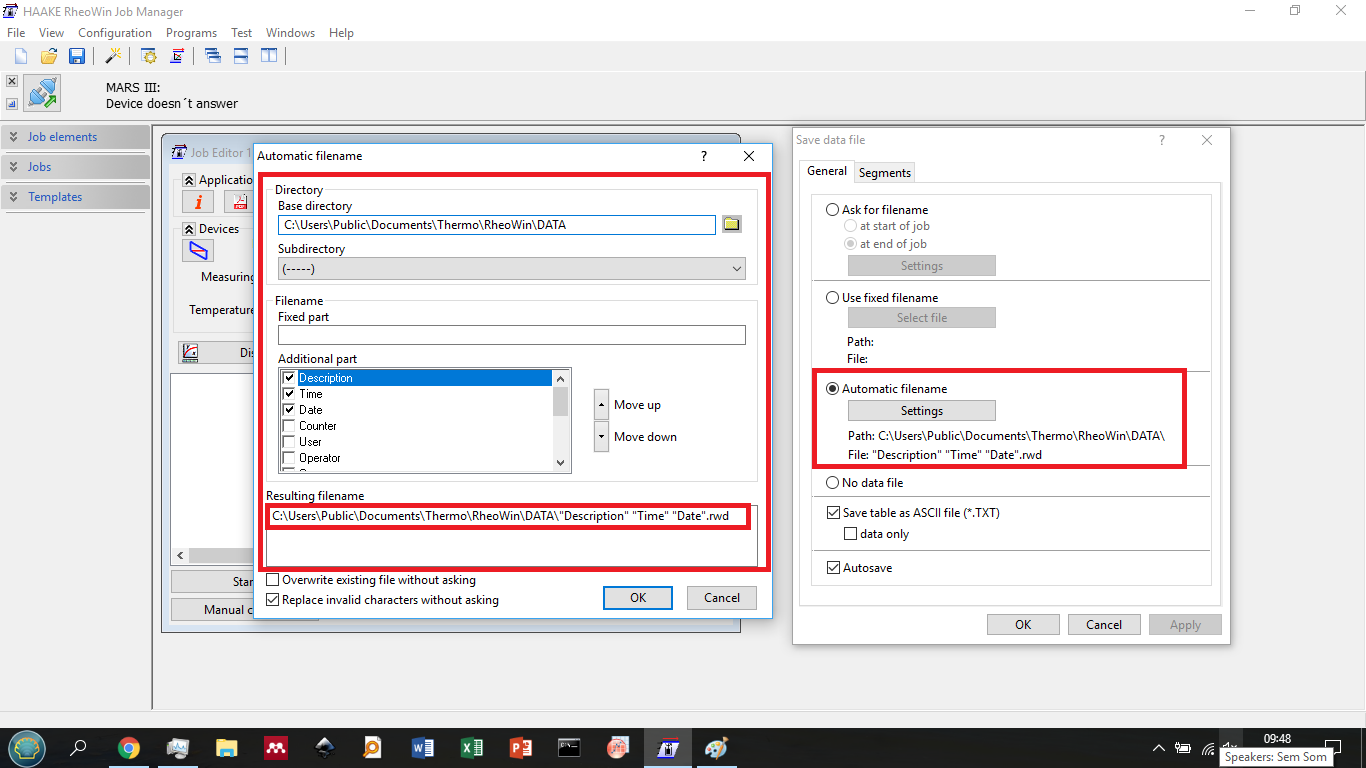
\includegraphics[width = 0.8\textwidth]{JobMan3}
\end{center}

\section{Configurando o Python}

Primeiramente, baixe o Python (3.6) do \href{http://python.org/}{python.org}. Clique em Downloads e depois selecione a versão mais nova para o Windows.

\begin{center}
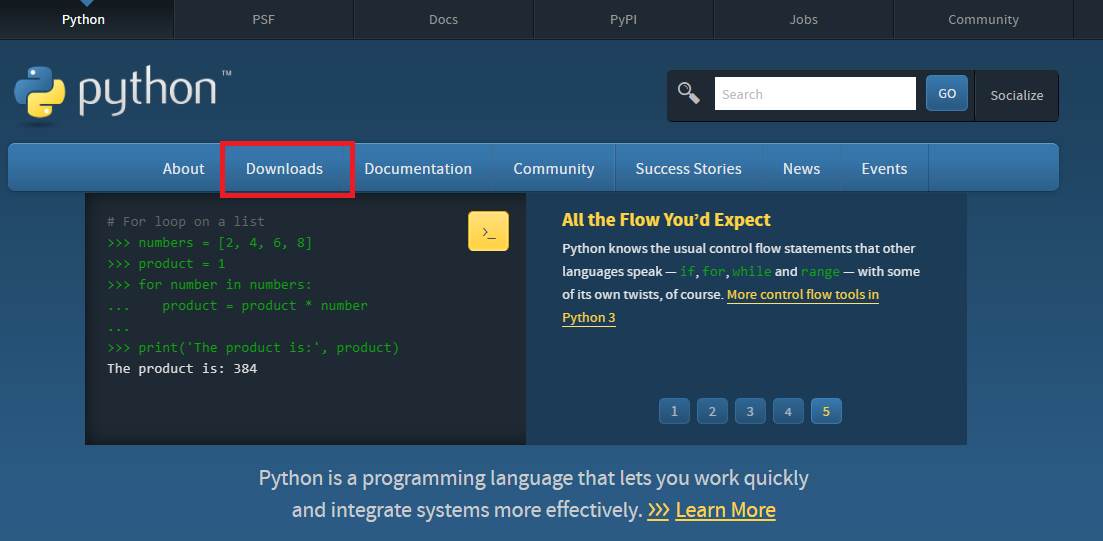
\includegraphics[width = 0.8\textwidth]{Pyt1}
\end{center}

\begin{center}
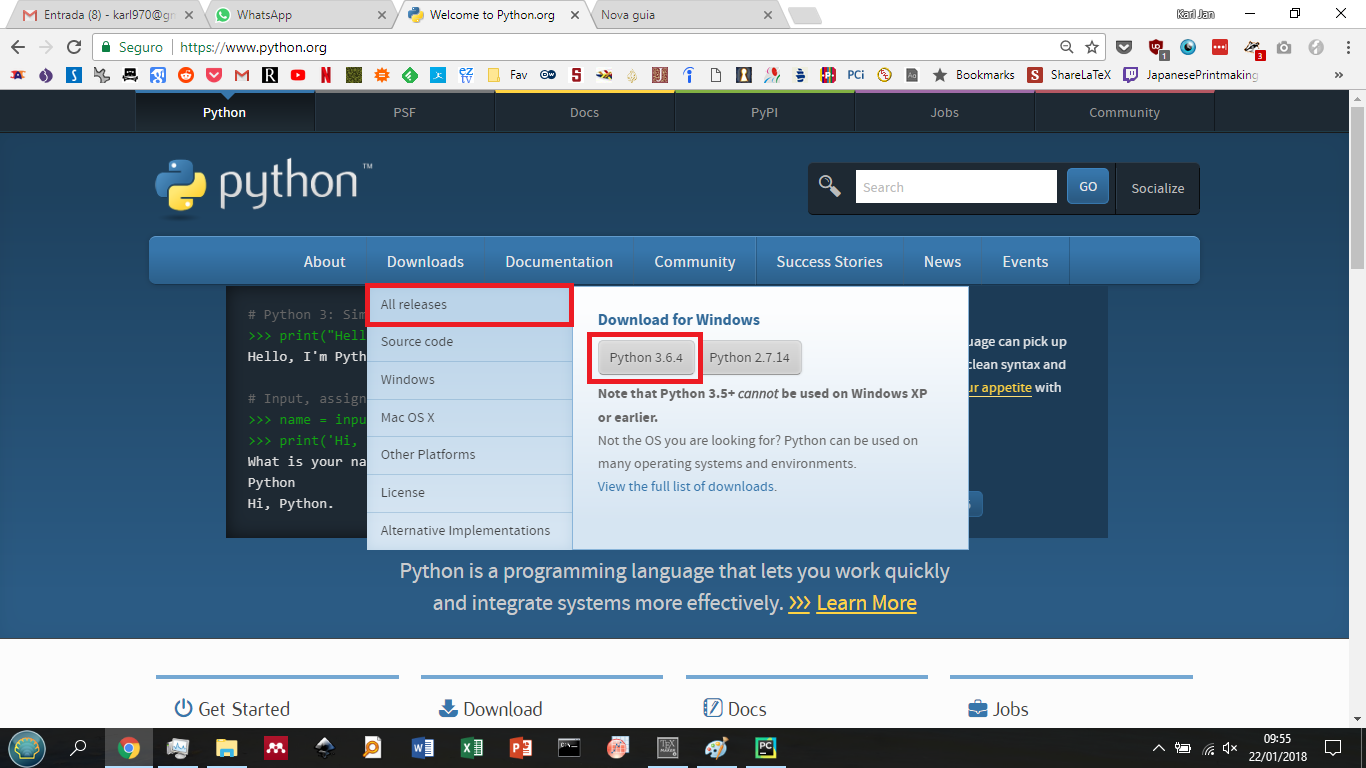
\includegraphics[width = 0.8\textwidth]{Pyt2}
\end{center}

Instale o Python. Selecione a instalação customizada e certifique-se do seguinte:

\begin{itemize}
\item \texttt{pip} está sendo instalado
\item python está sendo adicionado às variáveis de ambiente (\emph{Add Python to environment variables}).
\end{itemize}

Caso tenha dúvidas, siga \href{https://docs.python.org/3/using/windows.html}{\textbf{esta página}}.

\section{Baixando o script}

O script está no \href{https://github.com/KarlClinckspoor/Miscellaneous/tree/master/Rheology}{GitHub}. Os arquivos estritamente necessários são:

\begin{itemize}
\item RheoFC.py
\item requirements.txt
\end{itemize}

É recomendado que baixe também os arquivos:

\begin{itemize}
\item help
\item Readme.md
\end{itemize}

Coloque esses arquivos em uma pasta específica para o script. Depois que tudo está instalado, é necessário mover o arquivo \texttt{RheoFC.py} para a pasta com os arquivos \texttt{.txt} que contém os dados.

\section{Instalando os pacotes necessários}

Após o programa ter instalado, abra uma nova janela de comando ou do \emph{PowerShell} na pasta do script. Nessa pasta deverá haver o programa (\texttt{RheoFC.py}) e o arquivo \texttt{requirements.txt}. Abrir uma nova janela de comando na pasta atual pode ser feito clicando-se com o botão direito no Windows Explorer enquanto Shift está pressionado e depois clicar na opção de abrir uma janela de comando.

\begin{center}
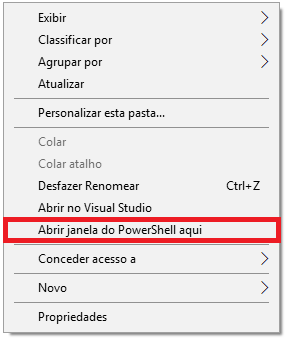
\includegraphics[width = 0.5\textwidth]{PowerShell}
\end{center}

Outra maneira de fazer isso é abrindo Executar (Com Windows + R), digitando \texttt{cmd} ou \texttt{powershell}, e depois navegando até o diretório desejado usando comandos \texttt{cd}.

Na pasta com o arquivo \texttt{requirements.txt}, digite:

\texttt{pip install -r requirements.txt}

O pip começará a instalar os arquivos necessários. Caso apareça um erro, dizendo que o comando não foi reconhecido, siga as instruções contidas \href{https://docs.python.org/3/using/windows.html}{aqui},  \href{https://stackoverflow.com/questions/3701646/how-to-add-to-the-pythonpath-in-windows-7}{aqui} ou \href{https://matthewhorne.me/how-to-install-python-and-pip-on-windows-10/}{aqui}.

Esta é a cara do script em andamento.

\begin{center}
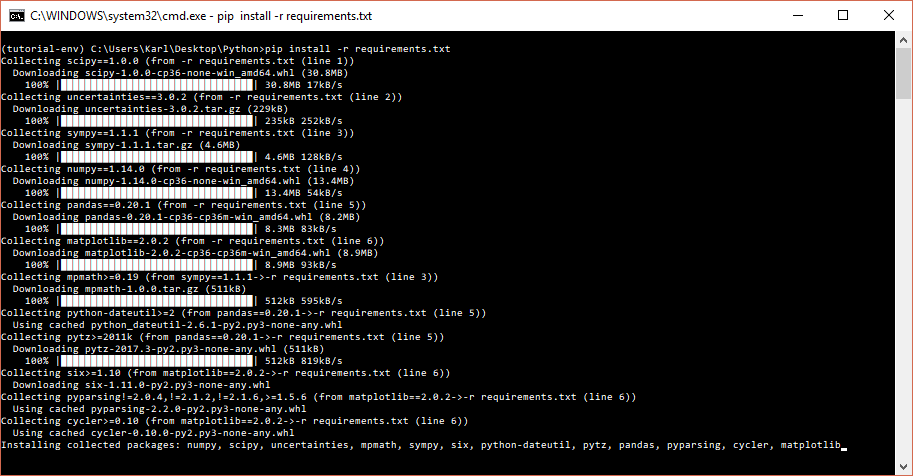
\includegraphics[width = 0.8\textwidth]{pip}
\end{center}

Esta é a transcrição de uma nova instalação pelo pip (em um ambiente virtual). 

\begin{footnotesize}
\begin{verbatim}

(tutorial-env) C:\Users\Karl\Desktop\Python>pip install -r requirements.txt
Collecting scipy==1.0.0 (from -r requirements.txt (line 1))
  Downloading scipy-1.0.0-cp36-none-win_amd64.whl (30.8MB)
    100% |████████████████████████████████| 30.8MB 17kB/s
Collecting uncertainties==3.0.2 (from -r requirements.txt (line 2))
  Downloading uncertainties-3.0.2.tar.gz (229kB)
    100% |████████████████████████████████| 235kB 252kB/s
Collecting sympy==1.1.1 (from -r requirements.txt (line 3))
  Downloading sympy-1.1.1.tar.gz (4.6MB)
    100% |████████████████████████████████| 4.6MB 128kB/s
Collecting numpy==1.14.0 (from -r requirements.txt (line 4))
  Downloading numpy-1.14.0-cp36-none-win_amd64.whl (13.4MB)
    100% |████████████████████████████████| 13.4MB 54kB/s
Collecting pandas==0.20.1 (from -r requirements.txt (line 5))
  Downloading pandas-0.20.1-cp36-cp36m-win_amd64.whl (8.2MB)
    100% |████████████████████████████████| 8.3MB 83kB/s
Collecting matplotlib==2.0.2 (from -r requirements.txt (line 6))
  Downloading matplotlib-2.0.2-cp36-cp36m-win_amd64.whl (8.9MB)
    100% |████████████████████████████████| 8.9MB 93kB/s
Collecting mpmath>=0.19 (from sympy==1.1.1->-r requirements.txt (line 3))
  Downloading mpmath-1.0.0.tar.gz (511kB)
    100% |████████████████████████████████| 512kB 595kB/s
Collecting python-dateutil>=2 (from pandas==0.20.1->-r requirements.txt (line 5))
  Using cached python_dateutil-2.6.1-py2.py3-none-any.whl
Collecting pytz>=2011k (from pandas==0.20.1->-r requirements.txt (line 5))
  Downloading pytz-2017.3-py2.py3-none-any.whl (511kB)
    100% |████████████████████████████████| 512kB 819kB/s
Collecting six>=1.10 (from matplotlib==2.0.2->-r requirements.txt (line 6))
  Downloading six-1.11.0-py2.py3-none-any.whl
Collecting pyparsing!=2.0.4,!=2.1.2,!=2.1.6,>=1.5.6 
(from matplotlib==2.0.2->-r requirements.txt (line 6))
  Using cached pyparsing-2.2.0-py2.py3-none-any.whl
Collecting cycler>=0.10 (from matplotlib==2.0.2->-r requirements.txt (line 6))
  Using cached cycler-0.10.0-py2.py3-none-any.whl
Installing collected packages: numpy, scipy, uncertainties, mpmath, sympy, six, 
python-dateutil, pytz, pandas, pyparsing, cycler, matplotlib 
 Running setup.py install for uncertainties ... done
  Running setup.py install for mpmath ... done
  Running setup.py install for sympy ... done
Successfully installed cycler-0.10.0 matplotlib-2.0.2 mpmath-1.0.0 numpy-1.14.0 
pandas-0.20.1 pyparsing-2.2.0 python-dateutil-2.6.1 pytz-2017.3
 scipy-1.0.0 six-1.11.0 sympy-1.1.1 uncertainties-3.0.2

(tutorial-env) C:\Users\Karl\Desktop\Python>
\end{verbatim}
\end{footnotesize}

\section{Rodando o script}

Após ter instalado todos os pacotes, rode o programa utilizando o comando \texttt{python RheoFC.py}. Ele irá carregar as configurações presentes, e depois você pode escolher o que deseja modificar. Quando terminar de configurar, ele iniciará o processo. Os dados do ajuste linear estarão no arquivo \texttt{linear.csv}, os dados do ajuste de Carreau no arquivo \texttt{Carreau.csv}, e assim por diante. Mais detalhes podem ser vistos no arquivo \texttt{Readme.md} (em inglês).

Exemplo:

\begin{center}
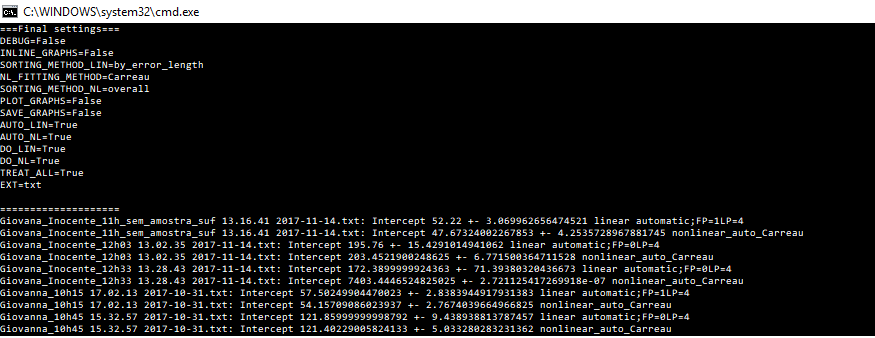
\includegraphics[width = 0.8\textwidth]{RheoFC1}
\end{center}

Pronto, parabéns, o script está funcionando. Bom proveito.
\end{document}